% code against the government vote
% produce a data.key
% how does Bundesrat decide on vote recommendation
% average sample size (and sd) 
% bias: overreporting of turnout, bandwaggoning, social desirability: it not socially desirable to vote for certain initiatives
% Is there underreporting of against the government votes?

\documentclass[11pt,a4paper]{article}\usepackage[]{graphicx}\usepackage[]{color}
%% maxwidth is the original width if it is less than linewidth
%% otherwise use linewidth (to make sure the graphics do not exceed the margin)
\makeatletter
\def\maxwidth{ %
  \ifdim\Gin@nat@width>\linewidth
    \linewidth
  \else
    \Gin@nat@width
  \fi
}
\makeatother

\definecolor{fgcolor}{rgb}{0.345, 0.345, 0.345}
\newcommand{\hlnum}[1]{\textcolor[rgb]{0.686,0.059,0.569}{#1}}%
\newcommand{\hlstr}[1]{\textcolor[rgb]{0.192,0.494,0.8}{#1}}%
\newcommand{\hlcom}[1]{\textcolor[rgb]{0.678,0.584,0.686}{\textit{#1}}}%
\newcommand{\hlopt}[1]{\textcolor[rgb]{0,0,0}{#1}}%
\newcommand{\hlstd}[1]{\textcolor[rgb]{0.345,0.345,0.345}{#1}}%
\newcommand{\hlkwa}[1]{\textcolor[rgb]{0.161,0.373,0.58}{\textbf{#1}}}%
\newcommand{\hlkwb}[1]{\textcolor[rgb]{0.69,0.353,0.396}{#1}}%
\newcommand{\hlkwc}[1]{\textcolor[rgb]{0.333,0.667,0.333}{#1}}%
\newcommand{\hlkwd}[1]{\textcolor[rgb]{0.737,0.353,0.396}{\textbf{#1}}}%

\usepackage{framed}
\makeatletter
\newenvironment{kframe}{%
 \def\at@end@of@kframe{}%
 \ifinner\ifhmode%
  \def\at@end@of@kframe{\end{minipage}}%
  \begin{minipage}{\columnwidth}%
 \fi\fi%
 \def\FrameCommand##1{\hskip\@totalleftmargin \hskip-\fboxsep
 \colorbox{shadecolor}{##1}\hskip-\fboxsep
     % There is no \\@totalrightmargin, so:
     \hskip-\linewidth \hskip-\@totalleftmargin \hskip\columnwidth}%
 \MakeFramed {\advance\hsize-\width
   \@totalleftmargin\z@ \linewidth\hsize
   \@setminipage}}%
 {\par\unskip\endMakeFramed%
 \at@end@of@kframe}
\makeatother

\definecolor{shadecolor}{rgb}{.97, .97, .97}
\definecolor{messagecolor}{rgb}{0, 0, 0}
\definecolor{warningcolor}{rgb}{1, 0, 1}
\definecolor{errorcolor}{rgb}{1, 0, 0}
\newenvironment{knitrout}{}{} % an empty environment to be redefined in TeX

\usepackage{alltt}
%\usepackage[utf8]{inputenc}
\usepackage{amsmath}
\usepackage{amsfonts}
\usepackage{amssymb}
\usepackage{graphicx}
%\usepackage[round]{natbib}
\usepackage[style=authoryear-comp,
natbib=true,
isbn=false,
url=false,
backend=bibtex]{biblatex}
\usepackage{url}
\usepackage{hyperref}
\usepackage{graphicx}
\usepackage{setspace}
\usepackage{booktabs}  
\usepackage{dcolumn} % alignment of colums along decimal point

%\bibliographystyle{apsrNoURL}
\bibliography{votingreferendums}

\author{Arndt Leininger \thanks{Hertie School of Governance, \texttt{a.leininger@phd.hertie-school.org}}}
\title{\Large{\textsc{Who votes against the government and why?}}\\ \large{\textsc{Voting Behavior in National Referendums in Switzerland}}} % Change title?
\date{\today}

\onehalfspacing
\IfFileExists{upquote.sty}{\usepackage{upquote}}{}
\begin{document}



\maketitle

{\small \textit{Contribution to the Leuven-Montréal Winter School in Elections and Voting Behaviour 2015. Current draft and code at:} \url{http://www.github.com/aleininger/votingreferendums}}



\begin{abstract}
  
	This paper studies voting behavior in national referendums in Switzerland, more concretely what motivates voters to vote counter to the vote recommendations issued by the Swiss federal government.
\end{abstract}	

\small\textbf{Keywords: Referendums, Voting, Switzerland, Multi-level modelling}

\vfill

\newpage

\section{Introduction}\label{sec:introduction}

    Voters vote in referendums more often and in more places than is commonly thought. Yet, voting in referendums has largely been a neglected topic in research on voting behavior which mostly focused on electoral behavior. The research that exists has focused on whether citizens are capable of casting an informed vote as levels of voter competence in referendums are thought to be even lower than in elections. This line of research has, counter to popular arguments against direct democracy, found that even uninformed citizens often are capable to vote in a way they would have voted had they been better informed on the issue at hand. Low-informed  voters are able to mimic informed voters' choices by relying on cues from governments, parties and interest groups.
    
    This paper is motivated by the observation that in Switzerland the effectiveness of such cues, concretely vote recommendations issued by the Swiss government, has apparently decreased. Switzerland has since roughly the late 1970s experienced a secular upward trend in the number of referendums the government loses, both in absolute and relative terms (Fig. \ref{fig}). In the past two legislative periods the government has lost at least 23\% of referendums while in the five periods before it has only lost 17.1\%. 
    The initiatives on a ban on building minarets in 2009 and the deportation of convicted non-Swiss citizens in 2010 which were both opposed by the government but still approved by a majority of voters are only two prominent examples from recent times. \footnote{The initiative Gegen den Bau von Minaretten'' was sponsored by politicians of the Swiss People's Party (SVP) and the Federal Democratic Union of Switzerland (EDU) and was brought to a vote on 29 November 2009. 57.5 and 19.5\% cantons voted in favor of it. 
    The initiative "Für die Ausschaffung krimineller Ausländer (Ausschaffungsinitiative)'', sponsored by the SVP, was brought to a vote on 28 November 2010 and was passed with 52.9\% and  
    17.5 voting in favor. } A more recent example is the anti-immigration initiative accepted by a slim majority of 50.3\% on 14 February 2014.
    
    I use the full cumulation of the VOX post-referendum surveys that cover 245 national referendums held in Switzerland between 1981 and 2010 (96.5 
    These surveys contain information on respondents’ voting behaviour, their personal characteristics as well as referendum-specific information.
    \% of the 254 referendums held in that period.) to analyze the individual and macro-level determinants of voting `against the government.' In the period considered the government issued 156 recommendations to vote yes, 97 and one neutral.\footnote{The latter is not included in the analysis because there is no vote recommendation that voters could vote against.} The type of referendum practically determines the recommendation the government will issue. As Obligatory Referendum is triggered by government action, requiring confirmation of parliamentary decisions by the people, the government has advocated for a yes-vote in all 61 obligatory referendums and obviously also for all its 18 counter-proposals to an initiative. The government also advocated a yes-vote in all but one of  76 facultative referendums. Note that in a facultative referendum voters are asked whether they approve of the law passed by parliament. The government advocated for a no in all but two initiatives of 99 referendums in total. Overall, in 49 (19.3\%) of referendums in that period a mjaority of voters did not follow the government's vote recommendation.  
    % lost referendums per decade absolute and relative
    
    \begin{table}[htb]
    \tiny\centering
      \begin{tabular}{lrrrr}
      \toprule
        & Obligatory Referendum & Facultative Referendum & Initiative & Counter-Proposal \\
      \midrule  
      Won & 51 (83.6\%) & 55 (72.4\%) & 90 (90.9\%) & 9 (50\%) \\
      Lost & 10 (27.6\%) & 21 (27.6\%) & 9 (9.1\%) & 9 (50\%) \\
      \bottomrule
      \end{tabular}
      
      \caption{Won and lost referendums by type.}
      
    \end{table}
    
    Given the state of the literature on referendum voting the paper is rather descriptive in nature. I focus on identifying possible determinants of the above defined outcomes rather than precisely estimating a specific determinant. As detailed in section \ref{sec:litreview} established determinants of electoral choice cannot be readily adapted to studies of vote choice in referendums and expected to work the same way. 
    
    On the individual level I concentrate on citizens' political competence -- capturing how informed voters are about a referendum -- and political sophistication more generally -- how interested and informed citizens are about politics in general. In include the usual socio-economic covariates which in Switzerland include the politico-linguistic divide between the German and the French and to a lesser degree the Italian speaking Swiss population. 
    
    On the macro level I spotlight the type and topic of a referendum. %as well as the campaign waged by proponents and opponents in the lead-up to a referendum. 
    While obligatory referendums are triggered by government action, initiatives are a tool for interest groups to enact policies the legislature would not pass. Who triggers a referendum could have an effect on citizens' propensity to reject the policy favored by the government. On the topics considered in a referendum it has been suggested by many commentators that initiatives directed against minorities have proven particularly successful. %Of particular relevance to parties and governments, lastly, is the question whether campaigns can encourage citizens to vote in the desired way.
    
    Following the presentation of initial results, I will also outline two potential extensions to the paper. Firstly, I articulate thoughts on how one could, among the voters `defying' the government, distinguish `reasoned' from `populist' deviators.Secondly, I discuss how an analysis of individual voting behavior could contribute to explaining the macro-level trend in rising numbers of government defeats. 
    
    This trend could be rooted in both macro and individual level factors. For instance, if voters are more likely to vote against the government's recommendation if the referendum was triggered by an initiative then the recent rise in initiatives on the ballot (Fig. \ref{fig}) could explain part of the increase in `defeats.' On the individual level, a decline in party identification in the voting population could explain why voters increasingly disregard their government's vote advice.

\begin{figure}[!htb]
% 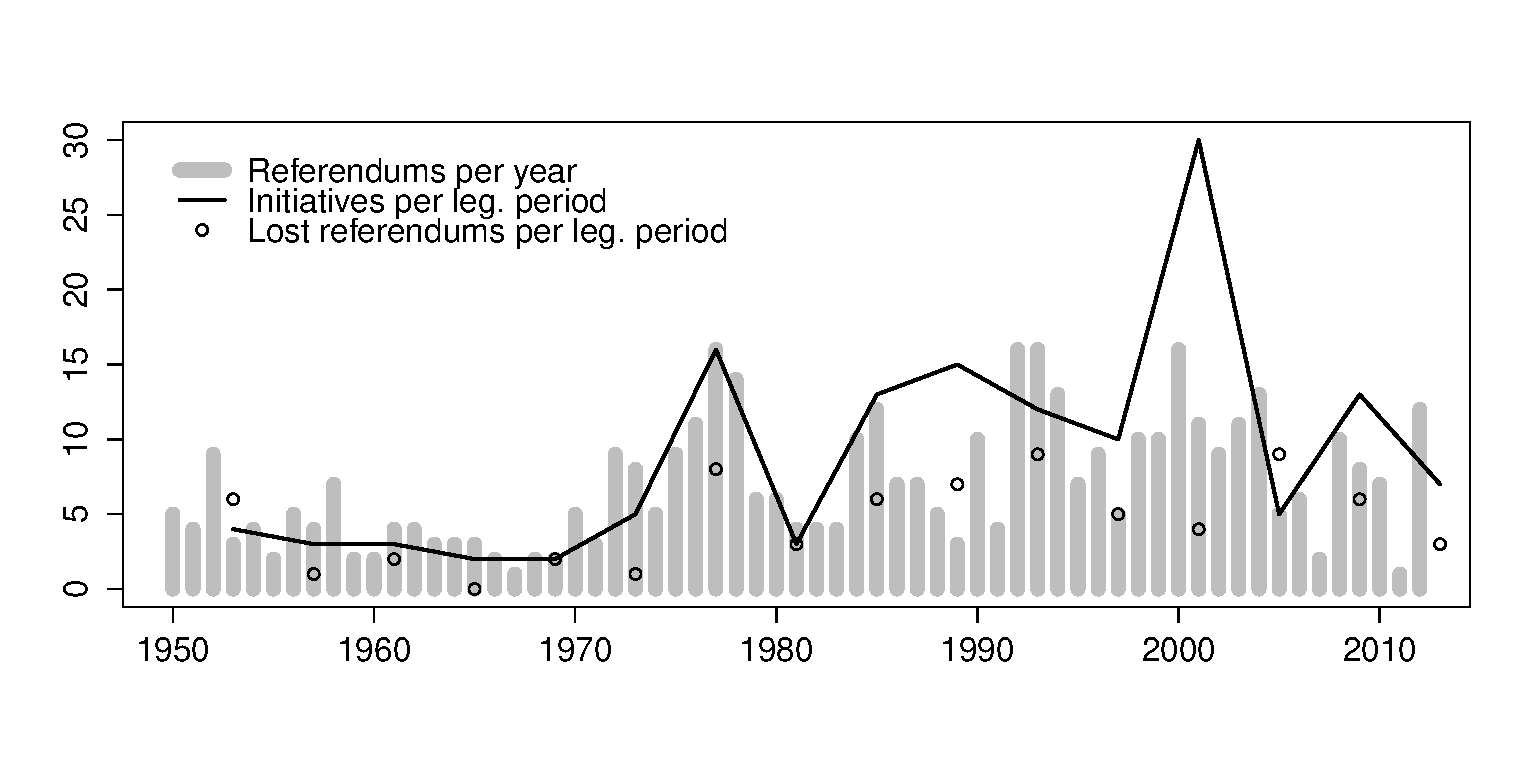
\includegraphics[width=\textwidth]{../../figures/figure.pdf}
\centering
\begin{knitrout}
\definecolor{shadecolor}{rgb}{0.969, 0.969, 0.969}\color{fgcolor}
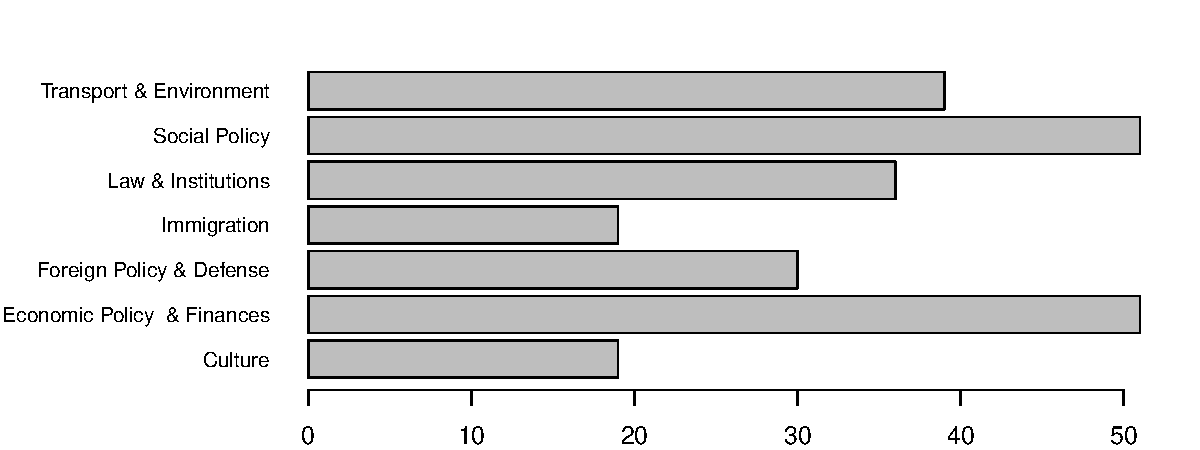
\includegraphics[width=\maxwidth]{figure/unnamed-chunk-1-1} 

\end{knitrout}
\caption{Number of national referendums, initiatives and referendums lost by the government in Switzerland (1950-2013). Counts per legislative period plotted at midpoint of legislative period.}\label{fig}
\end{figure}

\section{Literature review}\label{sec:litreview}

	The literature on voting behavior is immense with highly specialized sub-topics. literature reviews have to focus on the most immediately relevant papers in a given subfield of electoral behavior. 
	
	The literature on voting behavior largely is a literature of electoral behavior. The Oxford Handbook of Political Behavior contains no article on referendums. review much more scattered. odd collection of empirical cases outcomes of interest.
	
	Before providing a sketch of the literature, outline some of the reasons why referendums have received little attention in the voting literature. 
	
	substantive and practical reasons.
	
	Substantively, referendums have been of great appeal to theorists as embodiment of democracy, yet because of their lack of prominence in actual politics been of lesser interest. This has changed in recent years. increase in referendums globally. Extension of institutionalization. uptake in use and academic interest do not perfectly coincide as preliminary high point of use was in 90s(?). Greater role in politics, discussions of political reform. also explains academic interest.
		
Practical reasons. no data available. referendums occur infrequently and most often, outside of Switzerland, on the subnational level. Not many surveys. While every national and many subnational elections are accompanied by scientific election surveys scientific surveys on referendums are much rarer. Dalton and Klingemann say political behavior is a 'data-rich' field  of research (p. ?) However that is only true for 
	
	For this reason much research has been on aggregate level. Relating referendum outcomes to other macro level factors. not focus of this literature review which focuses on individual level.
	
	Schoen (2012) cautions that determinants of electoral and referendum participation differ, determinants of vote choice differ even more between elections and referendums. 
	
	Literature has (example attitudes towards international issues) focused on topic specific predictors.
	
	offers reasons:
	
%	"Solche von Bürgern initiierte Abstimmungen
%	beziehen sich häufig auf Forderungen, die in der repräsentativdemokratischen Arena keine
%	Mehrheit oder sogar überhaupt kein Gehör gefunden haben, und bringen insofern
%	Repräsentationsschwächen der zentralen repräsentativdemokratischen Akteure, also
%	vornehmlich der Parteien, zum Ausdruck. Daher ist es wohl kein Zufall, wenn bei
%	Volksentscheiden dieser Art andere politische Konfliktlinien und andere kollektive Akteure
%	als in der repräsentativdemokratischen Arena eine herausragende Rolle spielen" (Schoen 2012, S. 5)

referendums, initiatives, are used for proposal that found no majority in representative system or were not sufficiently addressed. referendums can be used by representative to 'outsource' contentious issues to the electorate. 

Other societal actors become more prominent. 

referendums vote on one issue as opposed to parties fundamentally different in essence. different context. regularities in electoral behavior cannot expected to appear in referendum voting.

even holds for strong determinants like party identification. If parties refrain from campaigning paty identification will play less role in determining vote choice. Schoen (2012) illustrates this where campaing was dominated by two interest groups.

Clark et al. speaking of referendums in Canada hold opposite standpoint party ID very important determinant of voting.



\section{Theory}\label{sec:theory}

referendums are not necessarily more difficult to put into an analytical framework that is amenable to a comparative and cumulative research agenda than elections.

if similiar topic they can be summarized. For instance eu integration. those referendums have been studied in comparative framework.

Here the proposal and proposer vary from referendum to referendum. 
Define an outcome variable that is consistent across referendums. Voting no, status quo bias. to a certain degree. but initiative no is pro status quo, in a facultative referendum not so clear, reversal of policy back to an older status quo. whether voters voted correctly. 

voters voted against government. normatively important. institution seems to be directed against representative process. a successful referendum is defeat for government. tool for populists.

normatively interesting.

take note of recent increase in government losses.

drawback of course is that it requires a government vote recommendation. Referendums
with no such recommendation can not be analyzed. Or one has to find other ways to
identify a government position.

Status quo bias. Voters are risk averse. Usually favors the government with the exception of obligatory referendums which are triggered by the government wishing to change the status quo.

Michigan: party identification issue and candidate orientation. 

there are no parties or candidates to elect, only an issue to decide. issue much more prominent. Party identification and 

every election is unique. voting research focuses on abstractions. voting for incumbent, for a left party, ticket-splitting. abstraction to be comparative and cumulative. but parties on offer are stable across elections. make sense to investigate vote choice for social democrats. develop an understanding how this might have changed. clear categories like government.

less expectations, more questions. 

\section{Questions}

Taking note of the recent increase in losses I seek answers to the question: what motivates citizens to vote against government? Voting behavior in referendums is little understood as outlined previous section.
My approach is descriptive in nature. I focus on identifying determinants of the above defined outcomes rather than precisely estimating a specific determinant. The partial correlations presented in section \ref{sec:results} should thus not be treated causal (Keele paper). For instance, the inclusion of political knowledge in the regression models is motivated by the normatively and politically important question whether voters are less well informed than others - holding other covariates constant. It is not motivated by the question whether lack of knowledge causes voting against the government. Consequently, I use the word partial correlation when referrring to coffiecient estimates. I do not use the word effect. 

probing relationships. it is not providing a theory and seeking to test it. Therefor, instead of formulating hypothesis I pose questions to motivate the use of the variables in the model. These are then followed by descriptions of the variable. A complete list of variables with descriptive statistics can be found in Appendix.

\textbf{Q} Are older citizens more likely to support the government's position?
Older citizens more likely to support the status quo. In the case of initiatives this implies opposing the initiative as it seeks to change the status quo. Initiatives are opposed by the government % is this the case for all initiatives?
- if the government were to support an initiative it would simply adopt the policies promoted by initiators leading them to abandon the initiative.
However, on obligatory referendums and facultative referendums the government advocates a no-vote % is this the case for all facultative referendums?
then preference for status quo would speak for voting against government.
Older citizens more trusting in government.

%\textbf{Q} Interaction effect between age and type

Education is important variable in referendum voting. educated are more confident about ability to participate why there support is not diminished by complicated decisison \citep{collingwood_levels_2012}. cuet taking % what does the literature say
normatively and empiricaly controversial questions of minority rights. direct democracy essentially majoritarian device. tyaranny of the majority. indeed, many votes on minority rightsin Siwtzerland and abroad. education important for voting on minority rights \citep{bowler_demanding_1998}. also in Swiss referendums \citep{vatter_who_2014} 

\textbf{Q} Are deviators less informed than voters voting with the government?



\section{Data \& Empirics}\label{sec:data}

inititally there are a total of %\Sexpr{} 
observations, when removing respondents who did not vote or cast an empty ballot the dataset reduces to %\Sexpr{} 
observations. Missing answers on some independent variables reduce the sample size further (see Tables %reference to regression tables
).

Observations ares clustered into referendums refered to as \textit{projets} and a referendum day -- on which voters may vote on multiple referendums -- referred to as \textit{scrutin}. 245 \textit{projets} clustered into 85 \textit{scrutins}. representative at the national level. 

One observation is not equivalent to one observations. as multiple referendums are held on one day, respondents about each referendum. Survey data are cumulated by referendum so that any single respondent appear to multiple observations, one for each referendum she participated in. 

cross-classified data. Respondents participated in multiple elections. referendums contain a number of respondents. Neither respondents are hierachically sorted into referendum, nor are referendums hierrachically sorted into respondents.

cross-classified random intercept model. 

multi-level models are now increasingly common in political science in general, and comparative survey research in particular. Prior comparative studies of political behavior (see section \ref{sec:litreview}) have also relied on two other approaches. Have estimated seperate regressions %citations here
, others have analyzed the data in one model, including dummies for the units of the contextual level 
\citep{eichenberg_europeans_1993}. The former approach is impractical for this paper. Would necessitate to estimate %\Sexpr{} 
regressions, one for each referendum. Dummy approach is effectively captures variance between higher-level units and focuses individual -level predictors on in this case within referendum-variance. However, not able to tell what is due to contextual factors and what to differences in level-1 variables. Also it precludes the estimation of context-level effects. 

From 1 to 6 projets per scrutin. On average 2.9 referendums per scrutin, median is 3.

Of these 98 are initiatives, NA are referendums, %facultative referendums?
NA are obligatory referendums, while %remainder category
\ref{fig:typetopic}.



average sample size of 580 (SD: 128)

\begin{figure}
\begin{knitrout}
\definecolor{shadecolor}{rgb}{0.969, 0.969, 0.969}\color{fgcolor}
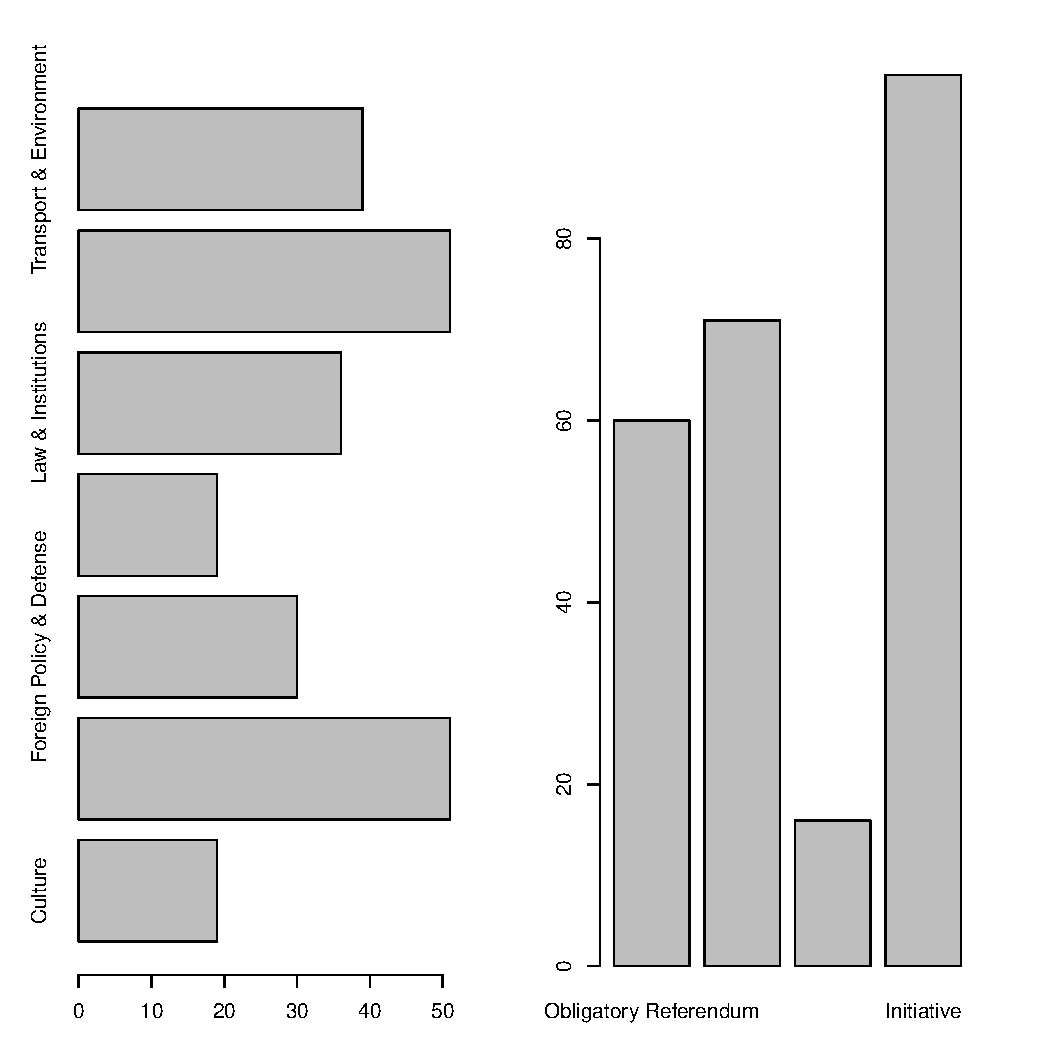
\includegraphics[width=\maxwidth]{figure/unnamed-chunk-2-1} 

\end{knitrout}
\caption{}\label{fig:typetopic}
\end{figure}

%As in most studies there is overreporting of turnout. Is there underreporting of against the government votes?

\section{Results}\label{sec:results}


\section{Conclusions}\label{sec:conclusions}

\textit{To be included in future revision.}

\printbibliography

\end{document}
